\chapter{One-Time-Pad und Schlüsseltausch}\label{ch:02}
Der Fortschritt in der Mathematik und das dazu gekommene Wissen machten Vigenère zu einem unsicheren Kryptosystem.
Vigenère und dessen Kryptoanalyse haben wir bereits besprochen. Wir haben gesehen, dass eine Kryptoanalyse vor allem dann leicht ist,
wenn der verwendete Schlüssel zu kurz gewählt wird, denn die wesentliche Schwäche
von Vigenère ist die Wiederholung der Muster im Kryptotext bei zu kurz gewähltem
Schlüssel. Betrachten wir als Beispiel einen Kryptotext aus 1000 Buchstaben, der mit einem Schlüssel der Länge fünf verschlüsselt ist. Das bedeutet, dass jeder fünfte Buchstabe und somit insgesamt je 200 Buchstaben anhand der gleichen Zeile der Vigenère-Tabelle
verschlüsselt sind. Das heisst, dass je 200 Buchstaben mit dem gleichen Schlüsselbuchstaben verschlüsselt sind. Durch eine Häufigkeitsanalyse von 200 Buchstaben kann ein
Kryptoanalytiker bereits den entsprechenden Buchstaben des Schlüssels bestimmen.
Was wäre aber, wenn der verwendete Schlüssel aus 50 Buchstaben bestehen würde?
Dann muss eine Häufigkeitsanalyse von 50 Teilen zu je 20 Buchstaben gemacht werden.
Es ist nicht garantiert, dass man aus nur 20 Buchstaben eine repräsentative Häufigkeitsverteilung erhält. Gehen wir noch einen Schritt weiter und wählen einen Schlüssel, der
genau gleich lang ist wie der Klartext. Nun ist eine Häufigkeitsanalyse völlig unmöglich,
da wir es mit 1000 Teilen zu je nur einem Buchstaben zu tun haben.

\begin{myprocedure}[Kryptosystem \gls{OTP}]\label{myprocedure:onetime}
	\leavevmode
	\begin{description}
		\item[Klartextalphabet:] Alphabet der lateinischen Grossbuchstaben.
		\item[Kryptotextalphabet:] Alphabet der lateinischen Grossbuchstaben.
		\item[Schlüsselmenge:] Alle denkbaren Texte bestehend aus lateinischen Grossbuchstaben, welche dieselbe Länge haben wir der Klartext. Es ist wichtig, dass für jeden Klartext ein Schlüssel zufällig generiert wird.
		\item[Verschlüsselung:] Gegeben ist ein zufällig gewählter Schlüssel $s$ aus der Schlüsselmenge. Der gegebene Klartext wird nun (wie gewohnt) mit Hilfe der Vigenère-Tabelle mit dem Schlüssel $s$ verschlüsselt. Der Schlüssel darf danach nicht mehr verwendet werden.
		\item[Entschlüsselung:] Gegeben ist ein zufällig gewählter Schlüssel $s$ aus der Schlüsselmenge. Der gegebene Kryptotext wird (wie gewohnt) durch Vigenère mit dem Schlüssel $s$ entschlüsselt.
	\end{description}
\end{myprocedure}

Warum erscheint uns das \gls{OTP} als ein sicheres Kryptosystem? Die Intuition ist
wie folgt. Weil der Schlüssel zufällig gewählt wird und genauso lang ist wie der Klartext,
wird jeder Buchstabe des Klartextes um zufällig viele Positionen im Alphabet verschoben.
Damit kann man den Kryptotext als eine zufällige Folge von Buchstaben betrachten. Und
aus einer zufälligen Folge von Buchstaben kann man keine Informationen herauslesen.

Alice und Bob haben sich in einem geheimen treffen schon vor einigen Tagen auf den geheimen Schlüssel der Länge 5 für das \gls{OTP} geeinigt. Alice verwendet nun den mit Bob vereinbarten Schlüssel, um eine geheime Nachricht (Kryptotext) an ihn zu senden. Der gesendete Kryptotext lautet \verb|GVRCL|.

Eva hat den Nachrichtenaustausch belauscht und somit den Kryptotext in Erfahrung
gebracht. Sie möchte nun den Klartext herausfinden um zu erfahren, was Alice und Bob
unternehmen werden. Eva vermutet, dass der Kryptotext mit dem sicheren \gls{OTP} verschlüsselt ist. Da der verwendete Schlüssel gleich lang ist wie der Klartext, ist eine Kryptoanalyse mit der Häufigkeitsanalyse unmöglich.

\begin{myexercise}
	\begin{aenum}
		\item Wie viele mögliche Schlüssel der Länge 5 gibt es?
		\item Kann Eve den Kryptotext \verb|GVRCL| entschlüsseln, falls sie (im schlimmsten Fall) alle Möglichkeiten durchprobiert?
	\end{aenum}
	\begin{myanswer}
		\begin{aenum}
			\item Es gibt $26^5 = 11'881'376$ verschiedene Möglichkeiten.
			\item Selbst wenn sie alle Schlüssel ausprobieren würde, gäbe es viele Klartexte die denkbar wären. Alice könnte nicht wissen, welches der tatsächliche Klartext ist.
		\end{aenum}
	\end{myanswer}
\end{myexercise}
Dennoch hat Eva das Gefühl, dass sie die geheime Nachricht erraten kann.
Die Anzahl aller Klartexte, die aus fünf Buchstaben einen sinnvollen Text ergeben, wird
vermutlich nicht so gross sein. Ausserdem weiss Eva, dass sich Alice und Bob verabreden
wollen. Eva listet deshalb einige sinnvolle Texte zu je fünf Buchstaben auf. Für jeden dieser
möglichen Klartexte bestimmt sie den Schlüssel (mit Hilfe der Vigenère-Tabelle), der den entsprechenden Text zu dem
gegebenen Kryptotext \verb|GVRCL| verschlüsseln würde.

\begin{table}[H]
	\centering
	\begin{tabular}{c|c}
		möglicher Klartext & entsprechender Schlüssel \\ \midrule\midrule
		BADEN              & FVOYY                    \\\midrule
		ESSEN              & CDZYY                    \\\midrule
		LESEN              & VRZYY                    \\\midrule
		SPORT              & OGDLS                    \\\midrule
		VIDEO              & LNOYX
	\end{tabular}
	\caption{Entsprechende Schlüssel bei geratenen möglichen Klartexten (BADEN, ESSEN, LESEN, SPORT, VIDEO) für abgehörten Kryptotext GVRCL.}
	\label{tab:GVRCL}
\end{table}
Jeder dieser Texte kann also durch den angegebenen Schlüssel zum Kryptotext \verb|GVRCL|
verschlüsselt werden. Welcher Text entspricht nun der richtigen Nachricht? Alice und Bob
haben ihren geheimen Schlüssel zufällig bestimmt, das heisst, jeder mögliche Schlüssel
kann mit der gleichen Wahrscheinlichkeit ausgewählt werden. Eva hat daher keine Möglichkeit herauszufinden, welche dieser vier möglichen Klartexte der geheimen Nachricht
entspricht. Es ist auch möglich, dass der richtige Klartext nicht in der Liste steht. Somit
hat Eva keine Chance irgendeinen Teil des Klartextes oder des Schlüssels zu erfahren.

\section{Kryptoanalyse bei mehrfacher Verwendung des Schlüssels}
Nun wollen wir wissen, weshalb ein Schlüssel beim \gls{OTP} nur einmal verwendet werden darf. Dazu schauen wir uns einen erneuten Nachrichtenaustausch zwischen
Alice und Bob an.
Alice möchte Bob nämlich eine weitere geheime Nachricht schicken. Da die zwei
jedoch zuvor keinen zweiten Schlüssel vereinbart haben, verwendet Alice den gleichen
Schlüssel ein zweites Mal. Diesmal erhält Bob von Alice den folgenden Kryptotext: \verb|ADRCM|.

Eva hat ihr Vorhaben, die beiden zu belauschen, noch nicht aufgegeben und versucht
erneut die verschlüsselte Mitteilung zu lesen. Wenn Alice und Bob für die zweite Nachricht einen neuen zufälligen Schlüssel ausgemacht hätten, dann könnte Eva erneut nichts mit dem Kryptotext anfangen. Alice war jedoch nachlässig und verwendete den gleichen
Schlüssel ein zweites Mal, um sich mit Bob zu verabreden.
Eva ergänzt ihre Tabelle mit einer dritten Spalte. In dieser Spalte notiert sie den Klartext,
der entsteht, wenn sie den zweiten Kryptotext mit dem entsprechenden Schlüssel aus der
zweiten Spalte entschlüsselt.
\begin{table}[H]
	\centering
	\begin{tabular}{c|c|c}
		möglicher Klartext & entsprechender Schlüssel     & möglicher Klartext für die zweite Nachricht \\ \midrule
		BADEN              & \textcolor{DarkGreen}{FVOYY} & \textcolor{Red}{VIDEO}                      \\
		ESSEN              & CDZYY                        & YASEO                                       \\
		LESEN              & VRZYY                        & FMSEO                                       \\
		SPORT              & OGDLS                        & FMSEO                                       \\
		VIDEO              & LNOYX                        & PQDEP
	\end{tabular}
	\caption{Entschlüsslung eines weiteren abgehörten Kryptotextes (ADRCM) durch die vorher bestimmten denkbaren Schlüsselkandiaten. Der Schlüsselkandidat FVOYY erzeugt aus beiden abgehörten Kryptotexten einen sinnvollen Klartext.}
	\label{tab:ADRCM}
\end{table}
\noindent
Und siehe da, fast alle Texte in der dritten Spalte ergeben keinen Sinn, ausser dem Text
in der ersten Zeile. Eva erkennt, dass mit dem Schlüssel FVOYY sowohl der erste wie auch
der zweite Kryptotext zu einem sinnvollen Text entschlüsselt werden können. Durch den
Vergleich der Entschlüsselungen des ersten und des zweiten Kryptotextes bei gleichem
Schlüssel konnte Eva die tatsächlichen Klartexte und den Schlüssel herausfinden.

\clearpage
\section{Bin-\gls{OTP}}
Das Kryptosystem Bin-\gls{OTP} funktioniert fast gleich wie das \gls{OTP}, nur dass wir nicht mit dem lateinischen Alphabet der Grossbuchstaben arbeiten wollen, sondern lediglich mit dem binären Alphabet $\lrc{0,1}$. Aus der grossen Vigenère-Tabelle in \cref{tab:vigenere} wird im binären Alphabet die übersichtliche (binäre) Vigenère-Tabelle:
\begin{figure}[H]
	\centering
	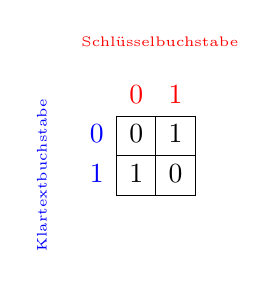
\begin{tikzpicture}
		\foreach \i in {0,...,1} {
				\node at (-0.5,-\i*0.5) {\textcolor{Blue}{\strut \i}};
				\node at (\i*0.5,0.5) {\textcolor{Red}{\strut \i}};
				\foreach \j in {0,...,1} {
						\edef\k{\ifnum\numexpr\i+\j\relax>1
								\the\numexpr\i+\j-2\relax
							\else
								\the\numexpr\i+\j\relax
							\fi}
						\node[draw,minimum size=0.5cm,inner sep=0pt]
						at (\i*0.5,-\j*0.5) {\strut\k};
					}
			}

		\node at (0.3,1.2) {\tiny{\textcolor{Red}{Schlüsselbuchstabe}}};
		\node[rotate = 90] at (-1.2,-0.5)  {\tiny{\textcolor{Blue}{Klartextbuchstabe}}};
	\end{tikzpicture}
	\caption{Vigenère-Tabelle für das binäre Alphabet.}
	\label{fig:VigenereBin}
\end{figure}
\noindent
Der Tabelle entnehmen wir, dass der Klartextbuchstabe $0$ durch den Schlüssel $0$ zum Kryptotextbuchstaben $0$ wird. Man verwendet für die Verschlüsslung mit der binären Vigenère-Tabelle eine besondere Schreibweise. Für die Verschlüsslung des Klartextbuchstaben $0$ durch den Schlüssel $0$ schreiben wir
\begin{align*}
	0 \oplus 0 = 0.
\end{align*}
Wird 0 durch 1 verschlüsselt erhalten wir den Kryptotextbuchstaben 1 (siehe Tabelle) und schreiben
\begin{align*}
	0 \oplus 1 = 1.
\end{align*}
Bitte beachten Sie, dass auch
\begin{align*}
	1 \oplus 0 = 1
\end{align*}
sowie
\begin{align*}
	1 \oplus 1 = 0
\end{align*}
gilt.
\noindent
Die Verschlüsslung mit dem binären \gls{OTP} erfolgt nun, indem Bit für Bit die Operation $\oplus$ (gemäss binärer Vigenère-Tabelle) durchgeführt wird. Analog haben wir mit den lateinischen Buchstaben auch die Verschlüsselung Buchstabe für Buchstabe mithilfe der Vigenère-Tabelle durchgeführt.

\begin{myexample}Folgendes Beispiel illustriert, wie die Verschlüsselung mit dem Bin-\gls{OTP} funktioniert:
\begin{itemize}
	\item
	      Der Klartext ist gegeben durch $\textcolor{Blue}{101}$ und der Schlüssel durch $\textcolor{DarkGreen}{111}$. Dann ist der Kryptotext gegeben durch
	      $\textcolor{Blue}{101} \oplus \textcolor{DarkGreen}{111} = \textcolor{Red}{010}$:
	      \begin{center}
		      \begin{tabular}{cccc}
			             & \textcolor{Blue}{1}      & \textcolor{Blue}{0}      & \textcolor{Blue}{1}      \\
			      \oplus & \textcolor{DarkGreen}{1} & \textcolor{DarkGreen}{1} & \textcolor{DarkGreen}{1} \\
			      \hline
			             & \textcolor{Red}{0}       & \textcolor{Red}{1}       & \textcolor{Red}{0}
		      \end{tabular}
	      \end{center}
	\item
	      Der Klartext ist gegeben durch $\textcolor{Blue}{011101}$ und der Schlüssel durch $\textcolor{Red}{110001}$. Dann ist der Kryptotext gegeben durch
	      \begin{align*}
		      \textcolor{Blue}{011101} \oplus \textcolor{DarkGreen}{110001} = \textcolor{Red}{101100}.
	      \end{align*}
\end{itemize}
\end{myexample}

\begin{myexercise}
	Berechnen Sie den Kryptotext zu dem gegebenen Klartext
	\begin{align*}
		110010100
	\end{align*}
	und zum Schlüssel
	\begin{align*}
		101110001.
	\end{align*}
	\begin{myanswer}
		Der Kryptotext lautet
		\[
		\begin{array}{r}
		110010100\\
		\oplus\;101110001\\
		\hline
		011100101
		\end{array}
		\].
	\end{myanswer}
\end{myexercise}

\begin{myexercise}
	\begin{aenum}
		\item Berechnen Sie sowohl
		\begin{align*}
			\textcolor{Red}{100110}\oplus \textcolor{Blue}{001011}
		\end{align*}
		als auch
		\begin{align*}
			\textcolor{Blue}{001011}\oplus \textcolor{Red}{100110}.
		\end{align*}
		Was stellen Sie fest?
		\item Seien $a$ und $b$ zwei beliebige Bits. Begründen Sie, warum stets die Gleichheit
		\begin{align*}
			a\oplus b = b\oplus a
		\end{align*}
		gilt. Wie heisst diese Eigenschaft?
	\end{aenum}
	\begin{myanswer}
		\begin{aenum}
			\item Wir berechnen
			\begin{align*}
				\textcolor{Red}{100110}\oplus \textcolor{Blue}{001011} = \textcolor{DarkGreen}{101101}
			\end{align*}
			sowie
			\begin{align*}
				\textcolor{Blue}{001011}\oplus \textcolor{Red}{100110} = \textcolor{DarkGreen}{101101}.
			\end{align*}
			In beiden Fällen erhalten wir dasselbe Resultat.
			\item Es gibt lediglich die 4 Fälle, welche wir der binären Vigenère-Tabelle entnehmen können. In den beiden Fällen $a = b = 0$ sowie $a = b = 1$ ist die Reihenfolge von $a$ und $b$ offensichtlich jeweils irrelevant, da sie identisch sind. In den beiden Fälle $a = 1$ und $b = 0$ sowie $a = 0$ und $b =1$ gilt
			\begin{align*}
				a\oplus b = 1\oplus 0 = 1 = 0\oplus 1 = b\oplus a.
			\end{align*}
			Damit sagt man, dass die Operation $\oplus$ \textit{kommutativ} ist. Die Reihenfolge der Operanden spielt bei der Operation $\oplus$ keine Rolle.
		\end{aenum}
	\end{myanswer}
\end{myexercise}

\begin{myexercise}
	Sei $a$ eine beliebige binäre Folge (denken Sie sich z.B. $a = 1100101$).
	\begin{aenum}
		\item Was macht die Verschlüsslung $a\oplus a$ von $a$ mit sich selbst?
		\item Mit $0$ bezeichnen wir im Folgenden eine Folge aus lauter Nullen derselben Länge wie $a$. Was macht die Operation $a\oplus 0$?
	\end{aenum}
	\begin{myanswer}
		Mit Hilfe der binären Vigenère-Tabelle begründen wir:
		\begin{aenum}
			\item $a\oplus a = 0$
			\item $a\oplus 0 = a$
		\end{aenum}
	\end{myanswer}
\end{myexercise}
Es lässt sich beweisen, dass die Operation $\oplus$ auch \textit{assoziativ} ist. Die Klammerung der Terme spielt also keine Rolle. Für beliebige binäre Folgen $a,b$ und $c$ derselben Länge gilt also
\begin{align*}
	(a\oplus b) \oplus c = a\oplus (b\oplus c).
\end{align*}
Dies gilt auch für mehr als drei Operanden.

\begin{myexercise}
	Es sei $t$ ein gegebener (binärer) Klartext. Alice wählt zufällig einen binären Schlüssel $s_A$ derselben Länge wie $t$ und berechnet
	\begin{align*}
		k_A := t\oplus s_A.
	\end{align*}
	Was erhält Alice, wenn sie nun
	\begin{align*}
		k_A\oplus s_A
	\end{align*}
	berechnet, also ihren Schlüssel erneut anwendet?
	\begin{myanswer}
		Sie erhält den Klartext $t$ zurück, denn
		\begin{align*}
			k_A\oplus s_A & =                                          \\
			              & (t\oplus s_A)\oplus s_A =                  \\
			              & t\oplus (s_A\oplus s_A) =                  \\
			              & t\oplus \underbrace{s_A\oplus s_A}_{= 0} = \\
			              & t\oplus 0 =                                \\
			              & t.
		\end{align*}
	\end{myanswer}
\end{myexercise}


\section{Schlüsseltausch}
\begin{figure}[H]
	\centering
	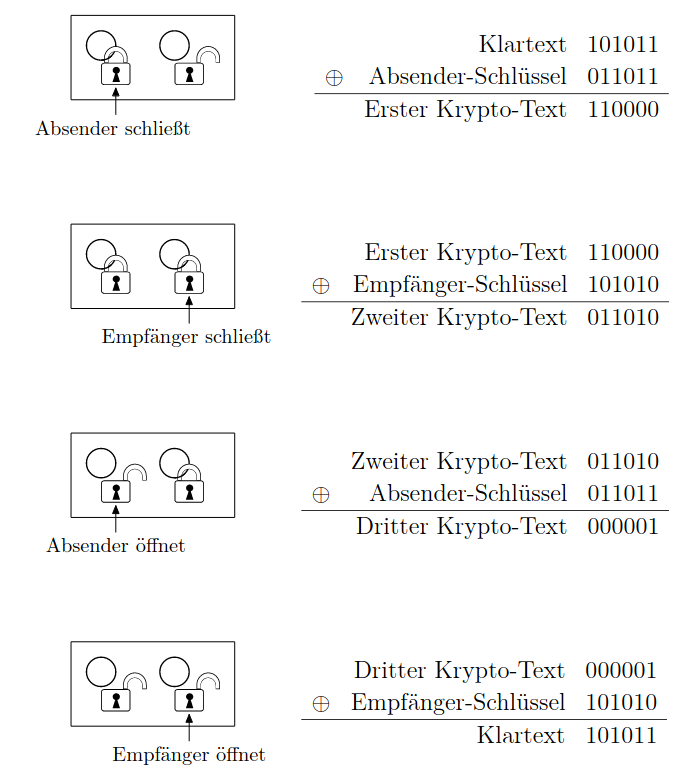
\includegraphics[width=0.7\textwidth]{Grundlagen_Info/03_Kryptologie/Figures/tausch.png}
	\caption{Schlüsseltausch}
	\label{fig:tausch}
\end{figure}

\clearpage
\begin{myprocedure}[Kommunikationsprotokoll Three-Pass Protocol]\label{myprocedure:Komm}
	Das Kommunikationsprotokoll Three-Pass Protocol (auch Schlüsseltausch mit drei Durchgängen genannt) ermöglicht es Alice, einen geheimen Schlüssel $t$ an Bob zu senden, ohne dass sie zuvor einen gemeinsamen geheimen Schlüssel vereinbart haben. Dazu verwenden sowohl Alice als auch Bob jeweils einen eigenen zufälligen Schlüssel ($s_A$ bzw. $s_B$).
	
	\begin{description}
		\item[Ausgangssituation:] Alice besitzt einen zufälligen binären Schlüssel $s_A$ der Länge $n$. Bob besitzt ebenfalls einen zufälligen binären Schlüssel derselben Länge $n$.
		\item[Ziel:] Alice hat zuvor einen geheimen binären Schlüssel $t$ der Länge $n$ gewählt. Diesen Schlüssel (das ist hier der Klartext) möchte sie über einen unsicheren Kanal an Bob senden, ohne dass Unbefugte den Schlüssel erfahren.
	\end{description}
	\begin{enumerate}
		\item \textbf{A}lice verschlüsselt den zu verschickenden Schlüssel $t$ (Klartext) mit ihrem Schlüssel $s_A$
		      \begin{align*}
			      k_A := t \oplus s_A
		      \end{align*}
		      und sendet den entstandenen Kryptotext $k_A$ an Bob.
		\item \textbf{B}ob verschlüsselt die empfangene Nachricht $k_A$ nun auch mit seinem Schlüssel $s_B$:
		      \begin{align*}
			      k_{AB} := k_A \oplus s_B
		      \end{align*}
		      und sendet den Kryptotext $k_{AB}$ zurück an Alice.
		\item Alice entschlüsselt den Kryptotext $k_{AB}$ mit ihrem Schlüssel $s_A$:
		      \begin{align*}
			      k_B = k_{AB} \oplus s_A
		      \end{align*}
		      und sendet $k_B$ an Bob.
		\item Schliesslich entschlüsselt Bob den Kryptotext $k_B$ mit seinem Schlüssel $k_B$:
		      \begin{align*}
			      t = k_B \oplus s_B
		      \end{align*}
		      und erhält dadurch den Klartext $t$, welchen ihn Alice wissen lassen möchte.
	\end{enumerate}
\end{myprocedure}
\noindent
Warum funktioniert das? Der Kern der Geschichte liegt darin, dass eine zweite Anwendung eines Schlüssels die erste Anwendung desselben Schlüssels löscht (rückgängig macht) und
zwar, auch wenn zwischen diesen zwei Anwendungen andere Schlüssel angewendet worden sind. Betrachten Sie die folgende Berechnung
\begin{align*}
	 & t\oplus s_A \oplus s_B\oplus s_A\oplus s_B =    \\
	 & t\oplus (s_A\oplus s_A)\oplus (s_B\oplus s_B) = \\
	 & t\oplus 0\oplus 0 = t.
\end{align*}

\begin{myexercise}
	Spielen Sie den Schlüsseltausch mit einer weiteren Person aus der Klasse durch.
	\begin{myanswer}
		\begin{itemize}
			\item Alice wählt den Schlüssel $s_A = 1011$ und den zu übermittelnden Schlüssel $t = 1100$.
			\item Bob wählt den Schlüssel $s_B = 0110$.
			\item Alice berechnet $k_A$ und sendet $k_A$ an Bob:
			\[
			\begin{array}{r}
			1100\\
			\oplus\;1011\\
			\hline
			0111
			\end{array}
			\]
			Also $k_A = 0111$.
			\item Bob berechnet $k_{AB}$ und sendet $k_{AB}$ an Alice:
			\[
			\begin{array}{r}
			0111\\
			\oplus\;0110\\
			\hline
			0001
			\end{array}
			\]
			Also $k_{AB} = 0001$.
			\item Alice berechnet $k_B$ und sendet $k_B$ an Bob:
			\[
			\begin{array}{r}
			0001\\
			\oplus\;1011\\
			\hline
			1010
			\end{array}
			\]
			Also $k_B = 1010$.
			\item Bob berechnet den Klartext-Schlüssel $t$:
			\[
			\begin{array}{r}
			1010\\
			\oplus\;0110\\
			\hline
			1100
			\end{array}
			\]
			Also $t = 1100$.
		\end{itemize}
	\end{myanswer}
\end{myexercise}


\subsection{Sicherheit des Drei-Wege-Schlüsseltauschs}
Ist das Drei-Wege-Kommunikationsprotokoll sicher? Bietet es dieselbe Sicherheitsgarantie wie die Verwendung einer Truhe mit zwei Schlössern? 

Wenn ein Kryptoanalyst nur einzelne Kryptotexte des Protokolls erhält und
das Verfahren nicht kennt, wirkt die Kommunikation als eine Folge von Zufallsbits und in diesem Sinne ist unsere Implementierung dieses Verfahrens sicher.  Wir müssen aber damit rechnen, dass der Gegner das Kommunikationsprotokoll kennt (oder erratet) und die zwei zufällig generierten Schlüssel das Einzige sind, was ihm unbekannt ist. 

Wenn der Gegner (Eve) alle drei Kryptotexte ($k_A, k_{AB}, k_B$) gewinnen kann, kann er durch die folgenden Berechnungen den Klartext $t$ herausfinden:
\begin{align*}
	& \textcolor{Red}{k_A} \oplus \textcolor{orange}{k_{AB}} \oplus \textcolor{yellow}{k_B} = \\
	& (\textcolor{Blue}{t} \oplus \textcolor{DarkGreen}{s_A}) \oplus (\textcolor{Red}{k_A} \oplus \textcolor{Purple}{s_B}) \oplus (\textcolor{orange}{k_{AB}} \oplus \textcolor{DarkGreen}{s_A}) = \\
	& (\textcolor{Blue}{t} \oplus \textcolor{DarkGreen}{s_A}) \oplus (\textcolor{Red}{k_A} \oplus \textcolor{Purple}{s_B}) \oplus ((\textcolor{Red}{k_A} \oplus \textcolor{Purple}{s_B}) \oplus \textcolor{DarkGreen}{s_A}) = \\
	& \textcolor{Blue}{t} \oplus (\textcolor{DarkGreen}{s_A} \oplus \textcolor{DarkGreen}{s_A}) \oplus (\textcolor{Purple}{s_B} \oplus \textcolor{Purple}{s_B}) \oplus (\textcolor{Red}{k_A} \oplus \textcolor{Red}{k_A}) = \\
	& \textcolor{Blue}{t} \oplus 0 \oplus 0 \oplus 0 = \\
	& \textcolor{Blue}{t}.
\end{align*}

\clearpage
\section{Diffie-Hellman-Merkle-Schlüsseltausch}
\begin{myprocedure}[Protokoll \gls{DHM})]\label{myprocedure:Diffie}
	Das Kommunikationsprotokoll \gls{DHM} ermöglicht es Alice und Bob, gemeinsam über einen öffentlichen Kanal einen geheimen Schlüssel zu vereinbaren, ohne dass sie zuvor einen gemeinsamen geheimen Schlüssel ausgemacht haben. Im Gegensatz zum Drei-Wege-Schlüsseltausch basiert das \gls{DHM}-Protokoll auf der Schwierigkeit, das diskrete Logarithmusproblem zu lösen, ein mathematisches Problem, zu dem es (bisher) keinen effizienten Lösungsalgorithmus gibt.
	\begin{description}
		\item[Ausgangssituation:] Alice und Bob haben sich zuvor öffentlich auf eine grosse Primzahl $p$ und eine positive natürliche Zahl $g$ geeinigt. Dabei ist $g$ kleiner als $p$.
		\item[Ziel:] Alice und Bob möchten gemeinsam mit einer öffentlichen Kommunikation einen Schlüssel $s_{AB}$ vereinbaren. Diesen Schlüssel darf keine Drittperson in Erfahrung bringen.
	\end{description}
	\begin{enumerate}
		\item Alice wählt zufällig eine positive ganze Zahl $a$ mit $a<p$ und hält diese geheim. Dann berechnet sie mit dieser geheimen Zahl:
		      \begin{align*}
			      x := g^a\mod p
		      \end{align*}
		      und sendet $x$ an Bob.
		\item Bob wählt zufällig eine positive ganze Zahl $b$ mit $b<p$ und hält diese geheim. Dann berechnet er die Zahl
		      \begin{align*}
			      y := g^b\mod p
		      \end{align*}
		      und sendet $y$ an Alice.
		\item Alice erhält $y$ von Bob und berechnet mit ihrer geheimen Zahl $a$ die Zahl
		      \begin{align*}
			      s_{AB} := y^a\mod p.
		      \end{align*}
		\item Bob berechnet mit dem erhaltenen $x$ und seiner geheimen Zahl $b$ die Zahl
		      \begin{align*}
			      s_{BA} := x^b\mod p.
		      \end{align*}
	\end{enumerate}
	Mithilfe der Rechengesetze der Modulo-Operation kann bewiesen werden, dass tatsächlich
	\begin{align*}
		s_{AB} = s_{BA}
	\end{align*}
	gilt und somit Alice und Bob dieselbe Zahl berechnet haben. Diese Zahl $s_{AB}$ ist der gemeinsame Schlüssel.
\end{myprocedure}


\begin{myexercise}
	Führen Sie das \gls{DHM}-Protokoll mit einer weiteren Person aus der Klasse durch. Verwenden Sie
	\begin{align*}
		p := 13 \quad \text{und}\quad g := 2
	\end{align*}
	(Sie können auch eigene Werte wählen) als öffentlich bekannte Schlüssel.
	\begin{myanswer}
		\begin{itemize}
		\item Alice wählt $a = 9$ und berechnet $x = 2^9 \mod 13 = 5$. Sie sendet $x = 5$ an Bob.
		\item Bob wählt $b = 10$ und berechnet $y = 2^{10} \mod 13 = 10$. Er sendet $y = 10$ an Alice.
		\item Alice berechnet den gemeinsamen Schlüssel: $s_{AB} = y^a \mod p = 10^9 \mod 13 = 12$.
		\item Bob berechnet den gemeinsamen Schlüssel: $s_{BA} = x^b \mod p = 5^{10} \mod 13 = 12$.
		\end{itemize}
		Alice und Bob haben somit denselben Schlüssel $s_{AB} = s_{BA} = 12$ vereinbart.
	\end{myanswer}
\end{myexercise}

\begin{myexercise}
	Versuchen Sie das Kommunikationsprotokoll \gls{DHM} zu knacken, indem Sie
	für die gegebenen Werte $p, g, x$ und $y$ jeweils die geheimen Zahlen $a$ und $b$ berechnen und daraus
	dann den vereinbarten Schlüssel $s_{AB}$.
	\begin{aenum}
		\item $g = 3, p = 5, x = 5, y = 2$
		\item $g = 2, p = 13, x = 6, y = 11$
	\end{aenum}
	\begin{myanswer}
		\begin{aenum}
			\item $a = 2, b = 3$ und $s_{AB} = 3^{2\cdot 3}\mod 5 = 4$
			\item $a = 5, b = 7$ und $s_{AB} = 2^{5\cdot 7}\mod 13 = 7$
		\end{aenum}
	\end{myanswer}
\end{myexercise}

\subsection{Sicherheit des \gls{DHM}-Protokolls}
Das \gls{DHM}-Protokoll ist sicher, weil es (bisher) keinen effizienten Algorithmus gibt, um das diskrete Logarithmusproblem zu lösen. Ein Kryptoanalyst (Eve) kann zwar die öffentlichen Werte $p, g, x$ und $y$ in Erfahrung bringen, aber um daraus den gemeinsamen Schlüssel $s_{AB}$ zu berechnen, müsste sie entweder die geheime Zahl $a$ von Alice oder die geheime Zahl $b$ von Bob bestimmen. Dies entspricht dem Lösen des diskreten Logarithmusproblems, was (bisher) als schwierig gilt.

Allerdings ist das DHM-Protokoll nicht gegen einen Man-in-the-Middle-Angriff geschützt. Ein Angreifer (Eve) könnte sich zwischen Alice und Bob schalten und so tun, als ob sie Alice wäre, wenn sie mit Bob kommuniziert, und umgekehrt. Dadurch könnte Eve sowohl mit Alice als auch mit Bob jeweils einen eigenen gemeinsamen Schlüssel vereinbaren und so die Kommunikation zwischen den beiden belauschen. Diese Schwäche kann durch die Verwendung von digitalen Signaturen behoben werden, welche die Authentizität der Kommunikationspartner sicherstellen. Ein Beispiel eines solchen Signaturverfahrens ist das \gls{RSA}-Kryptosystem (s. Kapitel \cref{subsec:rsa}).
